\PassOptionsToClass{
  title={Tensor Decomposition Notes},
  header,
  letterpaper,
  12pt
}{hw-scrartcl}

\documentclass{hw-scrartcl}

\usepackage{prob-style}
\usepackage{my-theorems}
%\usepackage{Latexmk}

\begin{document}
\maketitle
\section{Definitions and set-up}

Let's see if this works

Suppose that \(a_i \sim \Normal_d(0, I)\) are iid and define
\[
  T
  = \sum_{i=1}^n a_i^{\otimes k}.
\]

Given the entries of \(T\), we seek to recover the vectors \(a_i\) by optimising the objective
\[
  f(x)
  = \frac{1}{k}\sum_{i=1}^n \iprod{a_i}{x}^k
\]
under the constraint \(\norm{x} = 1\).

\subsection{Derivatives of \(f\)}
Take \(\tilde{\nabla}\) and \(\tilde{\nabla}^2\) to be the gradient and Hessian respectively of \(f\) on the sphere. Taking \(P_x = \Id - xx\transp\) to be the projection onto the subspace orthogonal to \(x\), we have the identities
\begin{align*}
  \tilde{\nabla} f(x)
  &= P_x \nabla f(x),\\
  \tilde{\nabla}^2 f(x)
  &= P_x \nabla \tilde{\nabla}f(x) P_x \\
  &= P_x \nabla^2 f(x) P_x - x\transp \nabla f(x) P_x.
\end{align*}

In particular, we have that
\begin{align*}
  \nabla f(x)
  &= \sum_{i=1}^n \iprod{a_i}{x}^{k-1} a_i,\\
  \tilde{\nabla} f(x)
  &= \sum_{i=1}^n \iprod{a_i}{x}^{k-1} P_x a_i,\\
  \tilde{\nabla}^2 f(x)
  &= (k-1) \sum_{i=1}^n \iprod{a_i}{x}^{k-2}P_x a_i a_i\transp P_x - \sum_{i=1}^n \iprod{a_i}{x}^k \Id_{d-1}.
\end{align*}

Now, write \(\alpha_i = \iprod{a_i}{x}\) and \(b_i = P_xa_i\) so that \(\alpha \sim \Normal_n(0, I)\) and \(b_i \sim \Normal_{d-1}(0, I)\) are mutually independent. We  can thus write that
\begin{align*}
  f(x)
  &= \sum_{i=1}^n \alpha_i^k, \\
  \tilde{\nabla} f(x)
  &= \sum_{i=1}^n \alpha_i^{k-1} b_i, \\
  \tilde{\nabla}^2 f(x)
  &= (k-1)\sum_{i=1}^n \alpha_i^{k-2} b_i b_i\transp - \sum_{i=1}^n \alpha_i^k \Id_{d-i} \\
  &= (k-1)\sum_{i=1}^n \alpha_i^{k-2} b_i b_i\transp - f(x)I_{d-1}.
\end{align*}

Hence, for any \(x\), \((f(x), \tilde{\nabla}f(x), \tilde{\nabla}^2 f(x))\) is mean \(0\) and can be describes with a function of independent standard Gaussians.

\subsection{Kac-Rice formula}
\begin{lemma}
  Lef \(f\) be a random function defined on the unit sphere \(s^{d-1}\)and let \(Z \subseteq S^{d-1}\). Under certain regularity conditions of \(f\) and \(Z\), we have, for \(\mathcal{M}_f\) the set of local maxima of \(f\),
  \[
    \E\abs{\mathcal{M}_f \cap Z}
    = \int_{S^{d-1}} \E[\abs{\det \tilde{\nabla}^2 f} \cdot \ind_{\tilde{\nabla}^2 f \preceq 0} \ind_{x \in Z} | \tilde{\nabla} f(x) = 0] p_{\tilde{\nabla} f(x)}(0) \diff x.
    \]
\end{lemma}

Conditioning on \(\alpha\), the quantity of interest thus becomes
\[
  h(\alpha)
  =  \E[\abs{\det \tilde{\nabla}^2 f} \cdot \ind_{\tilde{\nabla}^2 f \preceq 0} \ind_{x \in Z} | \tilde{\nabla} f(x) = 0, \alpha] p_{\tilde{\nabla} f(x)|\alpha}(0).
\]

We immediately have that
\[
  \tilde{\nabla} f(x) | \alpha
  \sim \Normal_{d-1}\Big(0, \sum_{i=1}^n \alpha_i^{2(k-1)}\Big),
\]
which renders
\[
  p_{\tilde{\nabla}|\alpha}(0)
  = \Big[\sum_{i=1}^n \alpha_i^{2(k-1)}\Big]^{(d-1)/2}
  = \norm{\alpha^{\odot (k-1)}}^{d-1}.
\]

\subsection{Useful Results}
\subsubsection{Shannon transform}
If \(A\) is an \(n\times n\) matrix whose largest eigenvalue is at most \(x\), then we have that, for \(m\) the Stieltjes stransform of \(A\),
\begin{align*}
  \int_x^\infty \Big(\frac{1}{w} + m(w)\Big) \diff w
  &= \int_x^\infty \int \Big(\frac{1}{w} + \frac{1}{\lambda - w}\Big) \diff \nu(\lambda) \diff w \\
  &= \int \int_x^\infty \frac{\lambda}{w(\lambda - w)} \diff w \diff \nu(\lambda) \\
  &= \int \log(1 - \lambda/x) \diff \nu(\lambda) \\
  &= \frac{1}{n} \log \det(\Id - A/x)
\end{align*}

\section{Conditioning in Kac-Rice}
Fixing \(x\) and \(\alpha\) conditioning on \(\tilde{\nabla} f(x) = 0\), and writing \(B = (b_1\vert \dotsb \vert b_n)\), we have that the entries of \(B\) are iid normals subject to the constraint
\[
  B\alpha^{\odot (k-1)} = 0.
\]

That is, the rows of \(B\) are iid normals supported on the \((n-1)\)-dimensional hyperplane orthogonal to \(\alpha^{\odot (k-1)}\). Hence, we have that
\[
  [B | \tilde{\nabla} f(x) = 0, \alpha]
  \deq [B(I - \bar{\alpha}\bar{\alpha}\transp) | \alpha],
\]
where \(\bar{\alpha} = \alpha^{\odot (k-1)}/\norm{\alpha^{\odot (k-1)}}\).

Now, conditionally on \(\alpha\), we can write, for \(P_\alpha = I - \bar{\alpha}\bar{\alpha}\),
\begin{align*}
  [\tilde{\nabla}^2 f(x) |  \tilde{\nabla} f(x) = 0]
  &= \Big[(k-1) B D_\alpha^{k-2}B\transp - f(x) \Id_{d-1} \Big| \tilde{\nabla} f(x) = 0\Big] \\
  &= (k-1) B P_\alpha D_\alpha^{k-2} P_\alpha B\transp - f(x) \Id_{d-1}.
\end{align*}

From the useful result, for \(k\) even, finding the log-determinant of this is equivalent to studying the spectrum of
\[
  D_\alpha^{k/2 -1} P_\alpha B\transp B P_\alpha D_\alpha^{k/2 - 1}.
\]

\section{Spectrum of the Hessian}

\begin{theorem}[Silverstein and Bai (1995)]
  Suppose that for each \(n\), the entries of \(\vec{X} = (\vec{x}_1, \dotsc, \vec{x}_n)\), \(p\times n\), are iid complex random variables with \(\E\abs{x_{11} - \E x_{11}}^2 = 1\), and that \(\vec{T} = \vec{T}_n = \diag(\tau_i^n, \dotsc, \tau_p^n)\), \(\tau_i^n\) real, and the ESD of \(\vec{T}\) converges almost surely to a probability distribution function \(H\) as \(n\rightarrow \infty\).

  Assume that \(\vec{B} = \vec{A} + \vec{X}^* \vec{T} \vec{X}\), where \(\vec{A} = \vec{A}_n\) is a Hermitian \(n\times n\) satisfying \(F^{\vec{A}_n} \vrightarrow F_\alpha\) almost surely, where \(F_\alpha\) is a distribution function (possibly defective, i.e., of total variation less than 1) on the real line. Furthermore, assume that \(\vec{X}, \vec{T},\) and \(\vec{A}\) are independent.

  When \(p/n \rightarrow y > 0\) as \(n\rightarrow \infty\), we have that almost surelt \(F^{\vec{B}}\), converges vaguely to a (non-random) d.f.\ \(\vec{F}\), whose Stieltjes transform \(m(z)\) is given by
  \begin{equation}
    \label{eqn:SilBai-stiltjes}
    m(z)
    = m_\alpha\Big(z - y\int \frac{\tau\diff H(\tau)}{1 + \tau m(z)}\Big).
  \end{equation}
\end{theorem}

\begin{theorem}
  For any \(z\) with \(\Im(z) > 0\), \cref{eqn:SilBai-stiltjes} has a unique solution \(m(z)\) which has positive imaginary part.
\end{theorem}

In the event that \(d/n \rightarrow \beta > 0\), the limiting EDF of \(\frac{1}{n} BDB\transp\) has Stiltjes transform \(m\) given implicitly by
\[
  -\frac{1}{m(z)}
  = z - \int \frac{s^{k-2}H(\diff s)}{1 + \beta s^{k-2} m(z)},
\]
where \(\phi\) is the standard normal pdf and \(H\) is the limiting empirical distribution of \(\alpha\).

In particular, for a finite but large \(n\), if we condition on \(\alpha\), treating \(D\) as deterministic, this renders the following approximation for \(m\):
\[
  -\frac{1}{m(z)}
  = z - \frac{1}{n}\sum_{i=1}^n \frac{\alpha_i^{k-2}}{1 + \beta \alpha_i^{k-2} m(z)}
\]


\section{Wishart Determinants}
\subsection{Joint density of Wishart eigenvalues}
Let \(M \sim \mathcal{W}_d(I, n)\) be a standard Wishart matrix. The eigenvalues of \(M\) then have joint density
\[
  Q_{n, d}(\lambda)
  = \frac{1}{Z_{n, d}} \prod_{i=1}^d \lambda_i^{(n-d-1)/2} e^{-\lambda_i/2} \prod_{i < j} \abs{\lambda_i - \lambda_j} \ind_{\lambda_1 \geq \dotsb \geq \lambda_d},
\]
where
\[
  Z_{n, d}
  = \frac{\pi^{d^2/2}}{2^{nd/2} \Gamma_d(n/2) \Gamma_d(d/2)},
\]
and in turn \(\Gamma_d\) is the multivariate gamma function defined by
\[
  \Gamma_d(a)
  = \pi^{d(d-1)/4} \prod_{i=1}^d \Gamma(a - (i-1)/2).
\]

\subsection{Determinant calculation}
Let \(x\) be a random variable independent of \(M\) with some density \(f\). We then have that
\begin{align*}
  \E[\abs{\det(xI - M)}
  &\ind_{(xI - M) \succeq 0} \ind_{x \in B}] \\
  &= \int_B f(x) \int_{x \geq \lambda_1 \geq \dotsb \geq \lambda_d} \prod_{j=1}^d (x - \lambda_j) Q_{n, d}(\lambda) \diff \lambda \diff x \\
  &= \frac{1}{Z_{n, d}} \int_B f(\lambda_{0}) \int_{\lambda_0 \geq \dotsb \geq \lambda_d} \prod_{0\leq i < j \leq d} \abs{\lambda_i - \lambda_j} \prod_{i=1}^d \lambda_i ^{(n-d-1)/2} e^{-\lambda_i/2} \diff \lambda \diff \lambda_0 \\
  &= \frac{Z_{n+1, d+1}}{Z_{n, d}} \int \lambda_0^{-(n-d-1)/2} e^{\lambda_0/2} f(\lambda_0)\ind_{\lambda_0 \in B} Q_{n+1, d+1}(\lambda) \diff \lambda \\
  &= \frac{Z_{n+1, d+1}}{Z_{n, d}} \E_{\mathcal{W}}^{n+1, d+1}\big[\lambda_{\max}^{-(n-d-1)/2} e^{\lambda_{\max}/2} f(\lambda_{\max}) ; \lambda_{\max} \in B\big]
\end{align*}

\section{Dynamics of gradient descent}
We can also write
\begin{align*}
  \tilde{\nabla}f(x)
  &= \sum_{i=1}^n \iprod{a_i}{x}^{k-1}a_i - x \sum_{i=1}^n \iprod{a_i}{x}^k \\
  &= \sum_{i=1}^n y_i^{k-1} a_i - x \sum_{i=1}^n y_i^k
\end{align*}
for \(y_i = \iprod{a_i}{x}\). Formally taking the time derivative through the gradient update step yields
\begin{align*}
  \dot{y}_j
  &= \iprod{a_j}{\dot{x}} \\
  &= \iprod{a_j}{\tilde{\nabla} f(x)} \\
  &= \sum_{i=1}^n y_i^{k-1}\iprod{a_i}{a_j} - y_j\sum_{i=1}^n y_i^k \\
  &= y_j^{k-1} \norm{a_j}^2 - y_j^{k+1} - y_j \sum_{i\neq j}y_i^k + \sum_{i\neq j} y_i^{k-1} \iprod{a_i}{a_j}.
\end{align*}

Further, taking \(w_j = y_j/\norm{a_j}\) so that recovery of \(a_j\) is characterised by \(w_j \rightarrow 1\), this becomes
\[
  \dot{w}_j
  = \norm{a_j}^k\bigg\{(w_j^{k-1} - w_j^{k+1}) - w_j \sum_{i\neq j} \Big[\frac{\norm{a_i}}{\norm{a_j}}\Big]^k w_i^k + \sum_{i\neq j} \Big[\frac{\norm{a_i}}{\norm{a_j}}\Big]^k w_i^{k-1} \frac{\iprod{a_i}{a_j}}{\norm{a_i}\norm{a_j}}\bigg\}.
\]

\subsection{Orthogonal case}
Before proceeding, we will consider the case where \(n \ll d\). This is very close to the orthogonal case, so first, let's consider the setting where the \(a_i\) are orthogonal unit vectors. The previous equations now become
\[
  \dot{w}_j
  = w_j^{k-1} - w_j^{k+1} - w_j \sum_{i \neq j} w_i^k.
\]

Notice that, since \(n \leq d\), we have
\begin{align*}
  1
  &= \norm{x}^2 \\
  &\geq \iprod{a_i}{x}^2 + \dotsb + \iprod{a_n}{x^2} \\
  &= w_1^2 + \dotsb + w_n^2.
\end{align*}

In particular, if \(w_j \rightarrow 1\), then \(w_i \rightarrow 0\) for all other indices \(i\). In particular, we have that \(\sum_{i\neq j}w_i^k \rightarrow 0\).

By flipping signs is necessary, we can assume that each \(w_j \geq 0\). Now, we have that, if \(w_j\) is the largest of the \(w\)s, then
\begin{align*}
  \dot{w}_k
  &= w_j^{k-1}(1 - w_j^2) - w_j \sum_{i \neq j} w_i^k \\
  &\geq w_j^{k-1}(1-w_j^2) - w_j^{k-1}\sum_{i\neq j} w_i^2 \\
  &\geq w_j^{k-1}(1 - w_j^2) - w_j(1 - w_j^2) \\
  &\geq 0.
\end{align*}

Hence, the largest \(w\) cannot decrease. In particular, is must converge. But now, solving \(\dot{w}_j = 0\) in the limit, we have
\[
  w_j^{k-1}(1 - w_j^2)
  = w_j \sum_{i\neq j} w_i^k.
\]

But the right-hand side is non-negative while the left is non-positive. Hence, we must have that \(w_j = 0\) or \(1\). But since \(w_j\) is the maximum \(w\), this means that \(w_j = 1\) and so the rest of the \(w_i = 0\). Hence, we conclude that the maximum \(w\) converges to \(1\) while the rest converge to \(0\). That is to say, after running gradient ascent, \(x \rightarrow a_j\).

\subsection{Undercomplete normal case}
Now, let's consider the \(a_i\)s again, though suppressing the inner product term. Suppose first that \(k = 3\). In this case, it is more interesting to study the quantity \(v_j(t) = \norm{a_j}^3 w_j\). The equations governing the \(v\)s are now
\[
  \dot{v}_j
  = v_j^2 - \frac{v_j^4}{\norm{a_j}^6} - v_j \sum_{i\neq j} \frac{v_i^3}{\norm{a_i}^6}.
\]

Now, suppose that \(v_j(t) = v_i(t) = \lambda\) for some \(i\neq j\) and \(t\). We then have that
\begin{align*}
  \dot{v}_j(t) - \dot{v}_j(t)
  &= -\frac{\lambda^4}{\norm{a_j}^6} + \frac{\lambda^4}{\norm{a_i}^6} - \lambda\sum_{l\neq j}\frac{v_l^3}{\norm{a_l}^6} + \lambda \sum_{l\neq i} \frac{v_l^3}{\norm{a_l}^6} \\
  &= \lambda^4\Big(-\frac{1}{\norm{a_j}^6} + \frac{1}{\norm{a_i}^6} + \frac{1}{\norm{a_j}^6} - \frac{1}{\norm{a_i}^6}\Big) \\
  &= 0.
\end{align*}

Hence, none of the \(v_j\) may cross each other. Hence, the greatest \(v_j\) stays the greatest.

Indeed, for any \(k\), this can be achieved for \(v_j = \norm{a_j}^\gamma w_j\) by taking \(\gamma = k/(k-2)\), as shown:
\begin{align*}
  \dot{v}_j
  &= v_j^{k-1} \norm{a_j}^{\gamma(2-k) + k} - v_j^{k+1} \norm{a_j}^{k(1-\gamma)} - v_j \sum_{i \neq j} \norm{a_i}^{k(1-\gamma)} v_i^k \\
  &= v_j^{k-1}  - v_j^{k+1}\norm{a_j}^{-2k/(k-2)} - v_j \sum_{i\neq j} v_i^k \norm{a_i}^{-2k/(k-2)}.
\end{align*}

Using a similar trick to the orthogonal case, we have thus that, for maximal \(v_j\),
\begin{align*}
  \dot{v}_j
  &\geq v_j^{k-1}(1 - v_j^2 \norm{a_i}^{-2\gamma}) - v_j^{k-1} \sum_{i\neq j} v_i \norm{a_i}^{-2\gamma} \\
  &= v_j^{k-1} \Big(1 - \sum_{i=1}^n w_j^2\Big).
\end{align*}

Now, notice that we have
\begin{align*}
  \deriv{}{t} \norm{w}^2
  &= 2\sum_{j=1}^n \dot{w}_j w_j \\
  &= 2\sum_{j=1}^n \Big[\norm{a_j}^k w_j^k(1 - w_j^2) - w_j^2 \sum_{i\neq j} \norm{a_i}^k w_i^k\Big] \\
  &= 2\sum_{j=1}^n \norm{a_j}^k w_j^k(1 - w_j^2) - 2\sum_{i=1}^n \norm{a_i}^k w_i^k \sum_{j\neq i}^n w_j^2 \\
  &= 2\sum_{j=1}^n \norm{a_j}^k w_j^k(1 - w_j^2) - 2\sum_{j=1}^n \norm{a_j}^k w_j^k(\norm{w}^2 - w_j^2) \\
  &= 2(1 - \norm{w}^2)\sum_{j=1}^n \norm{a_j}^k w_j^k,
\end{align*}
with equilibrium only when \(\norm{w} = 1\) or \(0\). Hence, if the sum is positive (especially for even \(k\)), we have that \(\norm{w} \rightarrow 1\).

Now, notice that, at \(\sum_{j=1}^n \norm{a_j}^k w_j^k = 0\), we have that
\begin{align*}
  \deriv{}{t} \sum_{j=1}^n \norm{a_j}^k w_j^k
  &= k\sum_{j=1}^n \norm{a_j}^k\dot{w}_j w_j^{k-1} \\
  &= k\sum_{j=1}^n \big[ \norm{a_j}^{2k}(w_j^{2(k-1)}  - w_j^{2k}) - \norm{a_j}^k w_j^k \sum_{i\neq j} \norm{a_i}^k w_i^k \\
  &= k\sum_{j=1}^n \norm{a_i}^{2k} w_j^{2(k-1)} - \Big(\sum_{j=1}^n \norm{a_j}^k w_j^k\Big)^2 \\
  &= k\sum_{j=1}^n \norm{a_i}^{2k} w_j^{2(k-1)} \\
  &\geq 0.
\end{align*}

Hence, the quantity \(\sum_{j=1}^n \norm{a_j}^k w_j^k\) can never switch from positive to negative. For odd \(k\), the sign of this quantity can be flipped simply by substituting \(x \mapsto -x\), so \(\norm{w}\) must converge for at least one of these options.

\subsection{Perturbation analysis}

\subsubsection{Failure in the overcomplete case}
\begin{figure}[p]
  \centering
  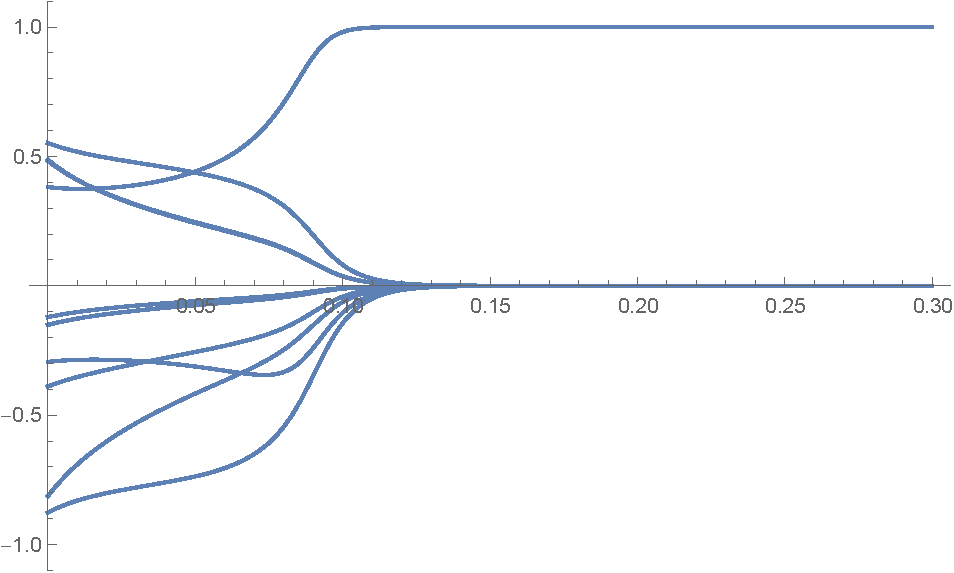
\includegraphics[width=\linewidth*2/3]{perturbation-analysis-failure/unperturbed.pdf}
  \vfill
  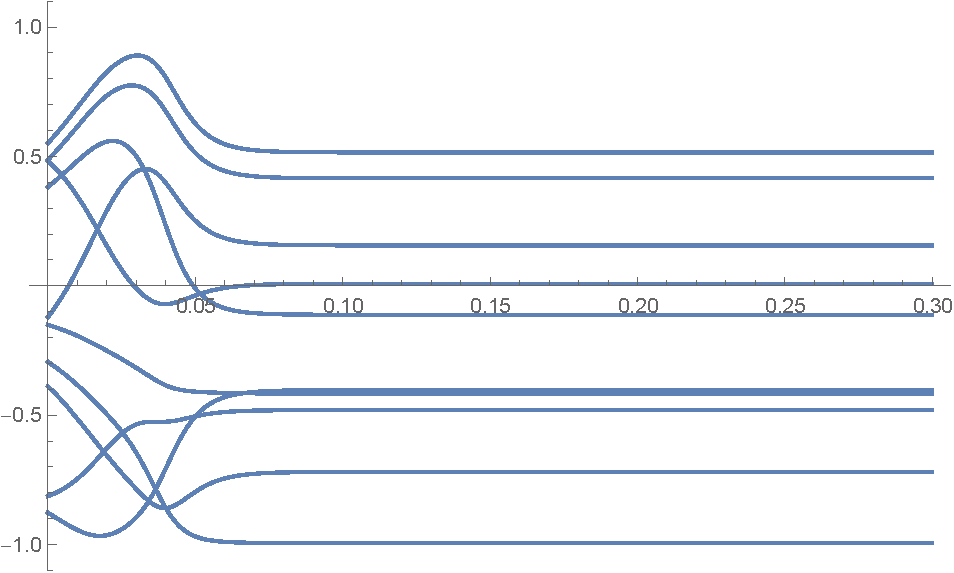
\includegraphics[width=\linewidth*2/3]{perturbation-analysis-failure/perturbed.pdf}
  \vfill
  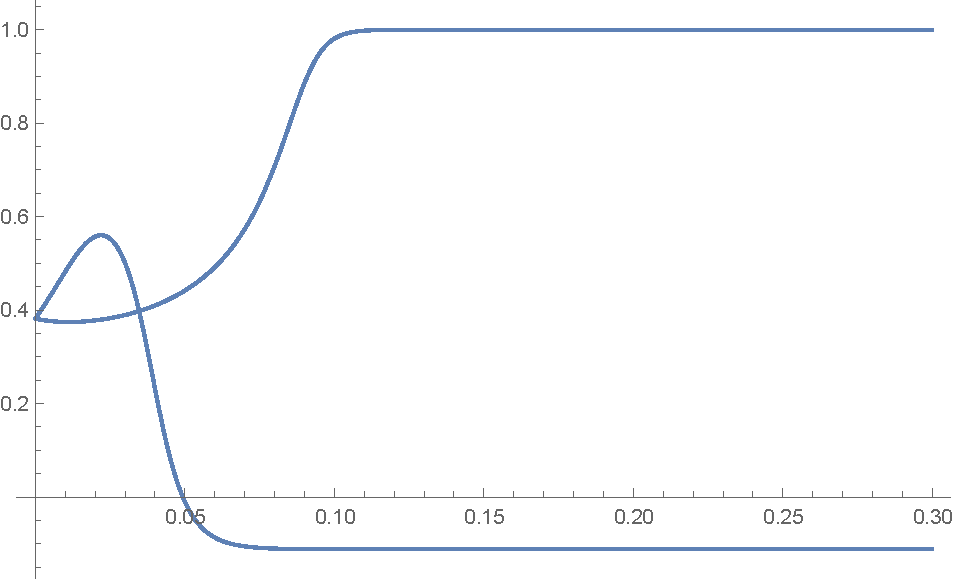
\includegraphics[width=\linewidth*2/3]{perturbation-analysis-failure/max-comparison.pdf}
  \caption{The unperturbed and perturbed systems, together with a comparison of the ``winner'' in the unperturbed case to the equivalent component in the perturbed case. \(n = 10, d=5, k=4.\)}
  \label{fig:perturbation-failure}
\end{figure}
Observe the plots in \cref{fig:perturbation-failure}, where the system has been simulated for \(n = 10, d=5, k=4\). We see that, as expected, in the unperturbed case, a single component ``wins,'' while the rest converge to \(0\). Unfortunately, when the system is perturbed, this component is not the eventual ``winner.''

\begin{figure}[p]
  \centering
  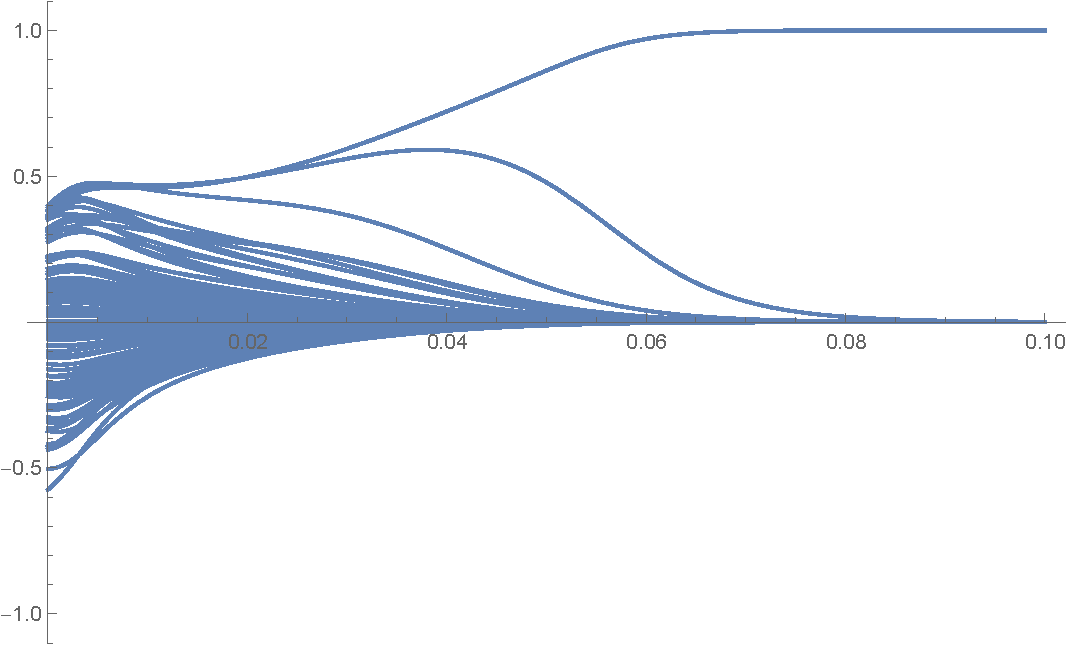
\includegraphics[width=\linewidth*2/3]{perturbation-analysis-failure/unperturbed-large.pdf}
  \vfill
  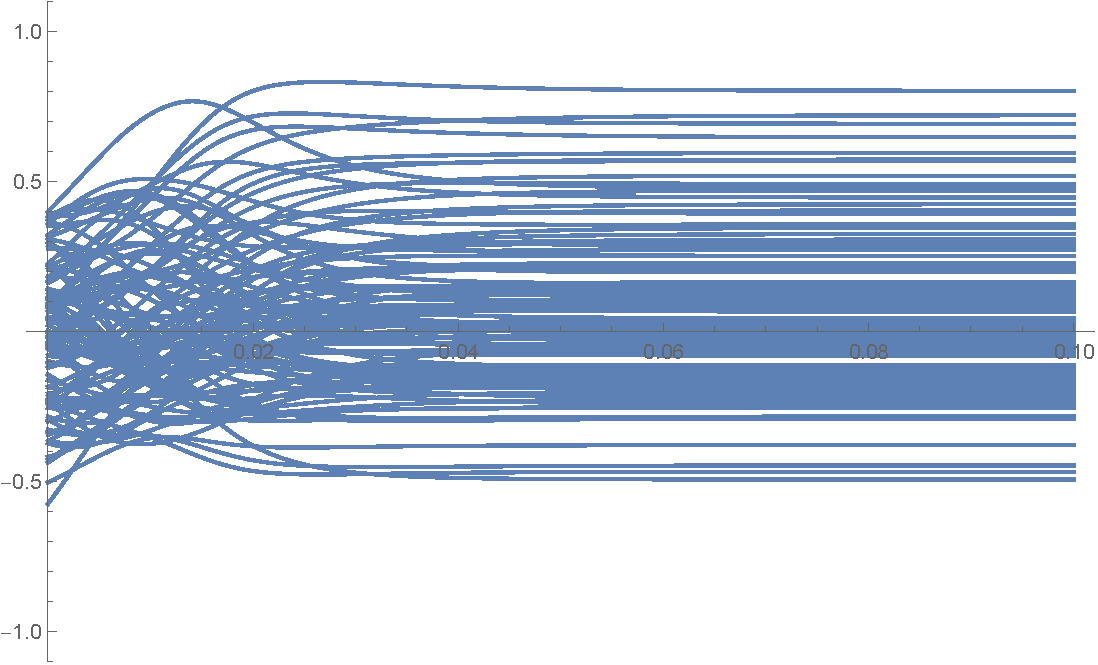
\includegraphics[width=\linewidth*2/3]{perturbation-analysis-failure/perturbed-large.pdf}
  \vfill
  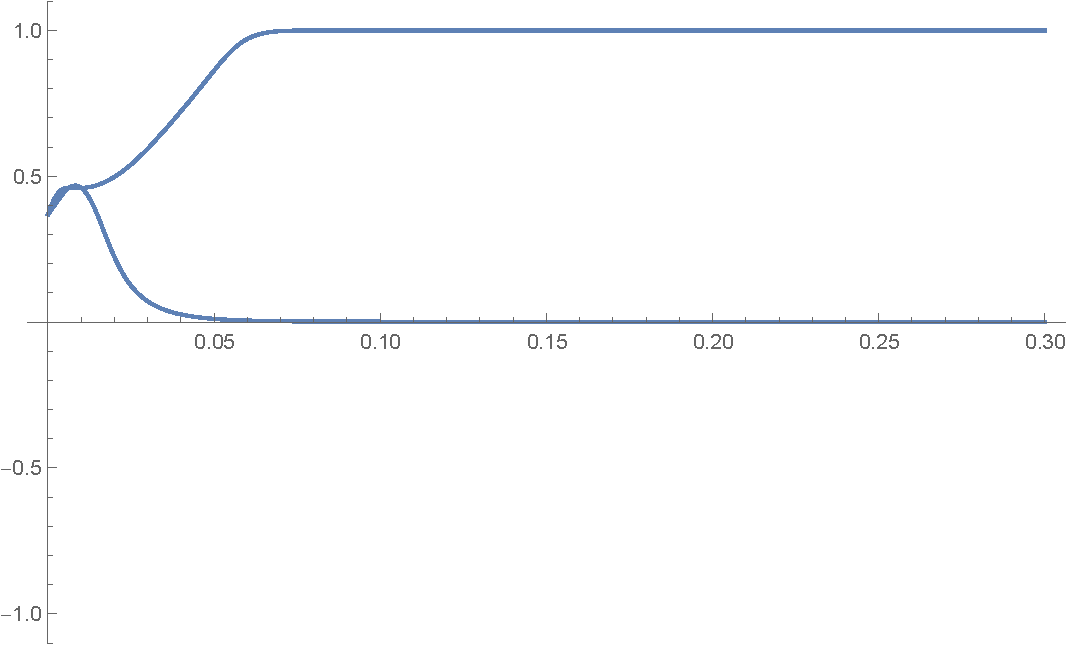
\includegraphics[width=\linewidth*2/3]{perturbation-analysis-failure/max-comparison-large.pdf}
  \caption{The unperturbed and perturbed systems, together with a comparison of the ``winner'' in the unperturbed case to the equivalent component in the perturbed case. \(n = 100, d=20, k=3.\)}
  \label{fig:perturbation-failure-large}
\end{figure}

However, all is not lost, since in the perturbed case, one of the components converges to a value close to \(-1\), and so a vector is recovered. However, as \(n\) grows large, the max value is not quite as good, as shown in \cref{fig:perturbation-failure-large} with \(n = 100, d=20, k=3\). Taking \(k = 4\) seems to solve this issue, likely because of the problem not getting ``stuck'' on the wrong side of the hemisphere.

\begin{figure}[p]
  \centering
  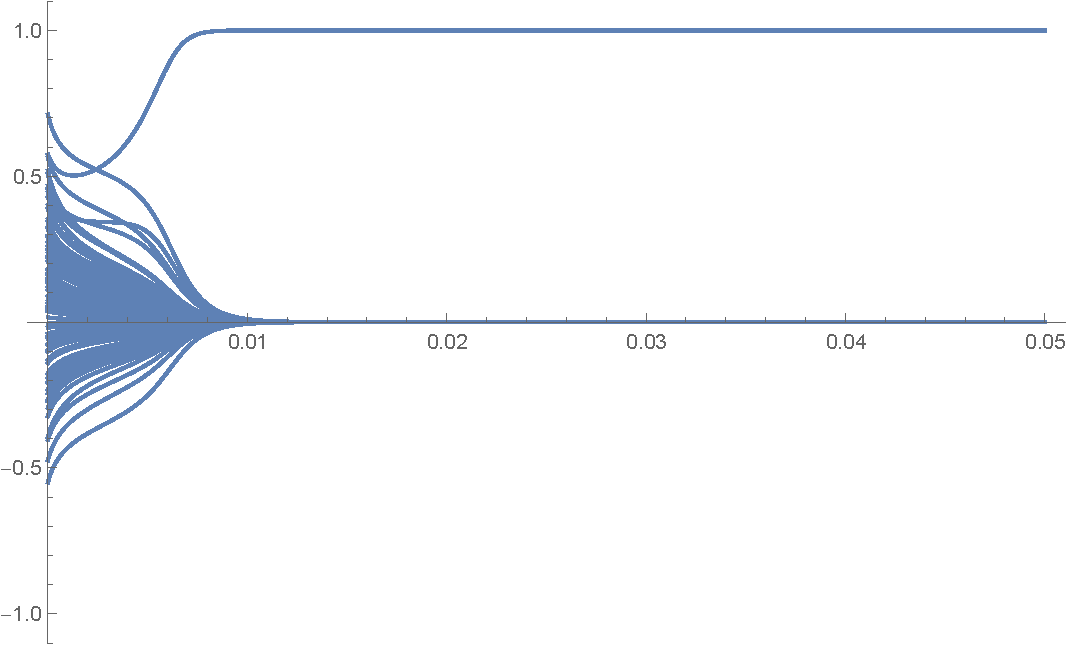
\includegraphics[width=\linewidth*2/3]{perturbation-analysis-failure/unperturbed-large-4.pdf}
  \vfill
  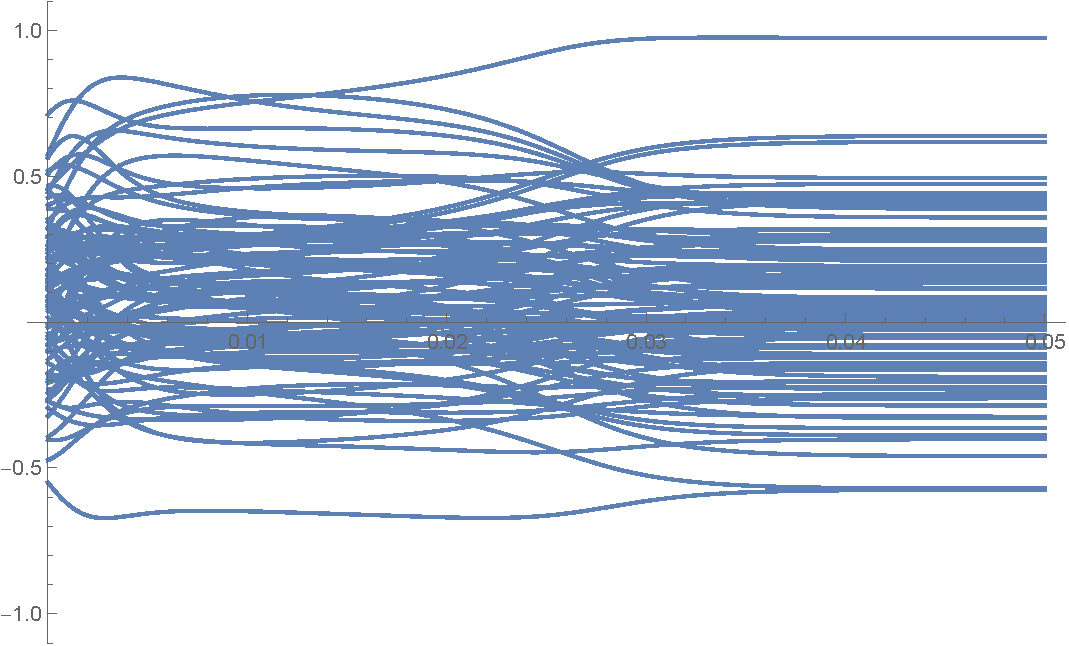
\includegraphics[width=\linewidth*2/3]{perturbation-analysis-failure/perturbed-large-4.pdf}
  \vfill
  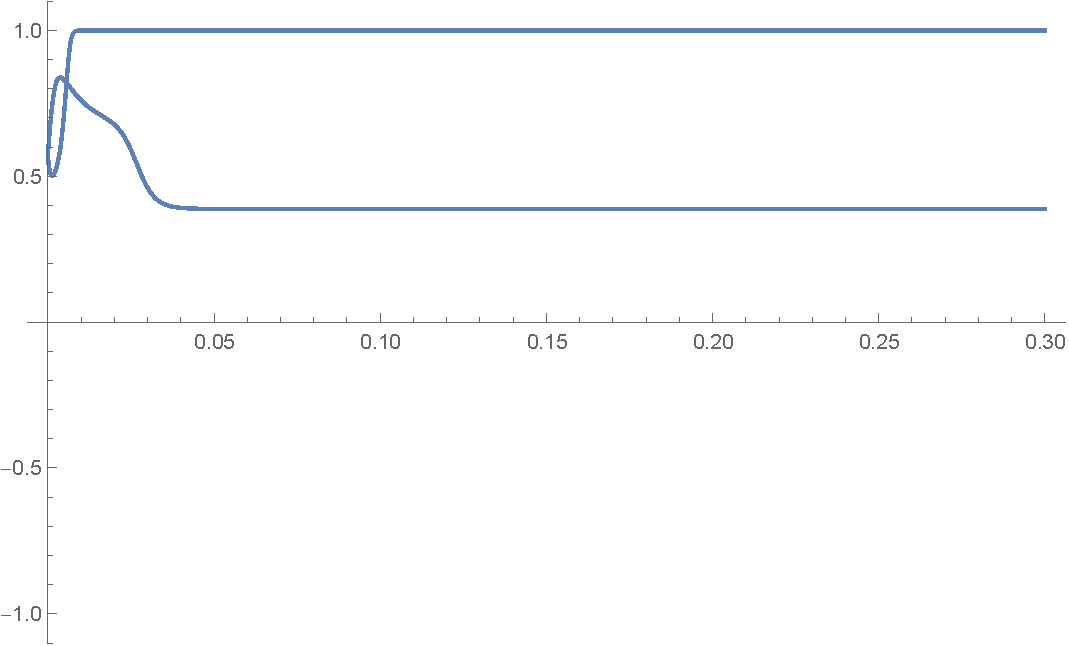
\includegraphics[width=\linewidth*2/3]{perturbation-analysis-failure/max-comparison-large-4.pdf}
  \caption{The unperturbed and perturbed systems, together with a comparison of the ``winner'' in the unperturbed case to the equivalent component in the perturbed case. \(n = 100, d=20, k=4.\)}
  \label{fig:perturbation-failure-large-4}
\end{figure}


\end{document}
